\secnumbersection{PROPUESTA DE SOLUCIÓN}
En este capítulo se entrega toda la información relacionada con la implementación y desarrollo de la solución. Este capítulo se divide en dos subcapítulos; en el primero se presenta el conjunto de tecnologías y una visión más detallada de la propuesta de solución. El subcapítulo siguiente se centra en aclarar y desarrollar ciertos detalles relevantes de la implementación.


\subsection{Descripción general de la solución}

\subsubsection{Conjunto de tecnologías}
El proyecto se desarrolla usando Python como lenguaje de programación y con el apoyo de librerías especializadas en computación científica y ciencia de datos como NumPy, SciPy, Pandas y Matplotlib. Para trabajar y manipular circuitos cuánticos vamos a utilizar la librería Pennylane\cite{pennylane}.  

La librería Pennylane forma parte del ecosistema de librerías especializadas en el control y la simulación de circuitos cuánticos, esta se diferencia de otras librerías, como Qiskit (desarrollada por IBM) y Cirq (desarrollada por Google), debido a su enfoque en la programación diferencial. Este enfoque permite desarrollar nuevos métodos que permitan ajustar sus parámetros, mejorando así su desempeño y generalidad (editando sus parámetros se pueden ajustar para mejorar su rendimiento en diferentes contextos).

En las siguientes secciones, cuando se hagan referencia a las funciones implementadas dentro de la librería, se utilizará la abreviación de \textit{qml}.

\subsubsection{Visión general del trabajo realizado}
Uno de los problemas de la librería es que implementa muchas funcionalidades y temas de interés, pero estas solo se presentan en modelos de juguete. La labor de software consiste en optimizar y utilizar estos conceptos y funcionalidades para crear modelos y estructuras más complejas.

Para lograr esto, se utiliza una programación con base en clases, estas se pueden agrupar en tres grandes tipos, hamiltoniano, \textit{ansatz} y optimizador (cada una construye objetos diferentes). La razón detrás de esta selección radica en buscar una independencia entre los componentes, en el flujo de los algoritmos variacionales cuánticos, de tal forma que los cambios en el tipo de hamiltoniano, \textit{ansatz}, etc. no genere una mayor repercusión dentro del código, más allá de los parámetros para construir de nuevo la clase. Para entender esto pensemos en que tenemos la clase del \textit{ansatz} UCCSD con la del optimizador genérico, la idea es que si queremos pasar de una estructura molecular al modelo de Fermi-Hubbard, solo tengamos que rehacer la clase del hamiltoniano mientras que la del \textit{ansatz} y optimizador quedan intactas.


El objetivo de la clase de los hamiltonianos es poder construirlo utilizando rutinas de la librería, además de, optimizar el cómo se agrupan los términos para una medición y ejecución de la función de coste más eficiente. La segunda clase se enfoca en crear el circuito y las características con las cuales se ejecutará (si tendrá un entorno con o sin ruido). Finalmente, la clase del optimizador, el cual es un objeto que almacena los hiperparámetros de los optimizadores disponibles en la librería.

A partir de lo anterior, es preciso tener en cuenta que este proyecto no busca ser otra librería que implemente piezas básicas para trabajar con circuitos cuánticos (como Qiskit, Cirq, Pennylane entre otros). Este proyecto pretende implementar flujos de cálculo complejos que permitan utilizar los métodos variacionales cuánticos para estudiar estructuras complejas.


\subsection{Detalles de la implementación}

\subsubsection{Hamiltoniano considerados}
El siguiente asunto es indicar con que hamiltonianos vamos a trabajar. Debido a que, como indicó en el marco teórico, tiene muchas formas de expresarse, considerando más o menos interacciones, por lo tanto, es importante aclarar que parámetros de los hamiltonianos se están considerando.

\begin{figure}[H]
\centering
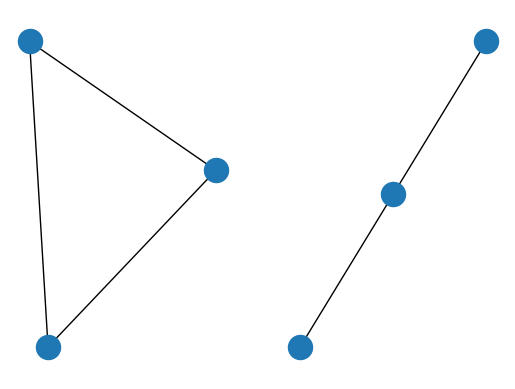
\includegraphics[width=0.5\textwidth]{figures/S3/condiciones.png}
\caption{\label{fig:CBorde} Grilla de estructura de anillo y cadena para 3 sitios respectivamente. Fuente: Elaboración propia}
\end{figure}

\underline{Hamiltoniano molecular}: 
Para el caso del hamiltoniano molecular, se consideran todas aquellas estructuras que pueden ser escritas en términos de elementos atómicos y sus correspondientes posiciones en el espacio, cabe destacar que las posiciones tienen que estar en unidades atómicas. 

Este hamiltoniano está en unidades de energía Hartree y es construido utilizando la función \textit{qml.qchem.molecular\_hamiltonian} (esta función construye el hamiltoniano de la ecuación \ref{eq:SCmolecular}). Para construir el hamiltoniano solo utilizamos el \textit{basis set} ''sto-3g''. El \textit{basis set} es un elemento fundamental en la construcción, ya que, en este, se encuentra la información de las constantes que acompañan los términos del hamiltoniano, ahorrando así tiempos de cálculos (considerando que estas constantes son integrales), el \textit{basis set} elegido corresponde a uno de los más básicos.

\underline{Hamiltoniano Fermi-Hubbard}: 
Para el hamiltoniano de Fermi-Hubbard, ver ecuación \ref{eq:FHHamiltonian}, consideramos las interacciones de \textit{hopping} ($-t$) y las del potencial ($-U$), no hay términos de interacciones externas (véase, un campo magnético y/o eléctrico). El hamiltoniano modela dos tipos de grilla (cadenas y anillos), ver figura \ref{fig:CBorde}.

De manera similar, como el hamiltoniano \textit{tight biding} se deriva del de Fermi-Hubbard considerando $U=0$, este está limitado a las mismas grillas.

La construcción de este hamiltoniano se realiza con las funciones \textit{qml.FermiA} y \textit{qml.FermiC} que implementan los operadores de aniquilación y creación respectivamente (operadores de segunda cuantización), y \textit{qml.jordan\_wigner} que permite después de construir el hamiltoniano en segunda cuantización pasarlo al espacio de espines. Él desafió de esta construcción utilizando estos operadores, poder es construir correctamente las interacciones dadas por las grillas.


\underline{Hamiltoniano espines}: 
Para el hamiltoniano de espines, ver ecuación \ref{eq:Heisenberg}, consideramos un modelo de Heisenberg con una interacción de \textit{exchange} ($J$) homogénea para cada eje, es decir, $J_{ij}^{x} = J_{ij}^{y} = J_{ij}^{z}$ $\forall i,j$ (este hamiltoniano es conocido en la literatura como \textit{quantum Heisenberg model XXX}). No se tiene en consideración campos externos. Este hamiltoniano modela dos tipos de grilla (cadenas y anillos), ver figura \ref{fig:CBorde}.

Este hamiltoniano se construye utilizando la función \textit{qml.pauli.string\_to\_pauli\_word}, que permite construir desde una lista de caracteres un operador, por lo tanto, al igual que en el hamiltoniano anterior, él desafió está en construir las listas que representen la acción de los operadores según la grilla elegida.

En lo que sigue del escrito, cuando se hagan referencia a los modelos, se debe tener en consideración las condiciones expresadas en este capítulo.

\subsubsection{Representación de los hamiltonianos}
Para almacenar los hamiltonianos descritos en el punto anterior, se elige escribirlos en la representación de lista de cadenas de Pauli. Si miramos la fórmula del cálculo del valor esperado (capítulo 2.4.2), no es necesario tener las matrices de forma explícita, como todo se mide respecto al eje Z, solo es necesario saber en qué índices de un término hay que aplicar un cambio de base para medirlo respecto al eje Z. Es por ello, que solo necesitamos un identificador de qué matriz de Pauli se está aplicando en cada sitio, para ello utilizamos el alfabeto $X$, $Y$, $Z$ y $I$, y representamos los términos como un solo \textit{string} compuesto por este alfabeto.

Para entender lo anterior, veamos un ejemplo, tomemos el término $\sigma_0^Z \otimes \sigma_1^Z \otimes \sigma_2^I$, matricialmente, esto es equivalente a una matriz de $8\times 8$, como no estamos utilizando las matrices y solo nos interesa los índices y el identificador, la matriz anterior puede ser representada como la siguiente cadena $''ZZI''$, en donde se refleja que en las primeras posiciones se tiene la acción del operador Z. En caso de tener alguna constante, esta se acopla como una lista, siguiendo el término de ejemplo, quedaría como $[-J, ''ZZI'']$.

Lo anterior es aplicado a cada término del hamiltoniano, permitiendo así una representación que reduce la cantidad de memoria requerida para almacenarla (al no tener que utilizar matrices de forma explícita) y a su vez mantiene toda la información necesaria para el cálculo de valores esperados.

%
%
%
%
%
\subsubsection{\textit{Ansatz} considerados}
Uno de los elementos fundamentales para trabajar con algoritmos variacionales cuánticos son los ansaztz. Para esta memoria consideramos tres \textit{ansatz} de estructura fija, el UCCDS, el k-UpCCGSD y el HE, los cuales serán utilizados en el VQE para estimar el estado y valor de mínima energía.

\underline{UCCDS}:
El primer \textit{ansatz} corresponde al UCCSD, el cual está compuesto por operadores de excitación simples y dobles, estos operadores mantienen constante el número de partículas. Este \textit{ansatz}, por su estructura, no tiene la capacidad de aplicar repeticiones (adjuntar el mismo \textit{ansatz} varias veces dentro del circuito). Este se encuentra implementado en la función \textit{qml.UCCSD}.


\underline{k-UpCCGSD}: 
El segundo \textit{ansatz} se basa en la misma teoría que el anterior (\textit{Unitary Coupled Cluster}), este también se define basándose en operadores de excitación simples y dobles (por lo tanto, también conserva el número de partículas constante), con el detalle de este si admite la posibilidad de generar $k$ repeticiones dentro del circuito. Este se encuentra implementado en la función \textit{qml.kUpCCGSD}


\underline{\textit{Hardware Efficient}}: 
El concepto de \textit{Hardware Efficient} es muy amplio, ya que, hace referencia a compuertas nativas al \textit{hardware}, para esta memoria consideramos una implementación que es afín a hamiltonianos hermíticos, esta se basa en compuertas de rotación $R_Y(\theta)$ y compuertas $CX$, ver figura \ref{fig:RY}. Este \textit{ansatz} es conocido en la literatura como ''\textit{Real amplitudes}'', ya que, al manejar solo esa rotación, estamos dando a entender que los estados solo tendrán amplitudes reales. Ambas compuertas están implementadas en \textit{qml.ry} y \textit{qml.cnot}.

\begin{figure}[H]
\centering
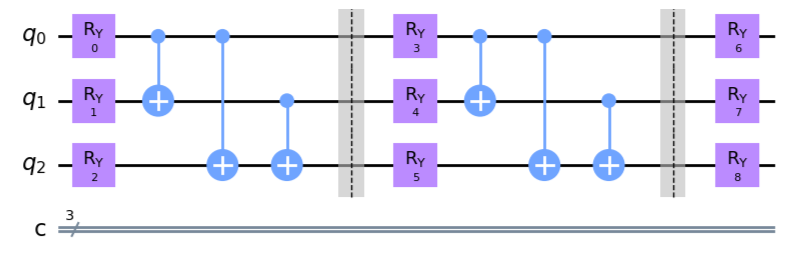
\includegraphics[width=0.8\textwidth]{figures/S2/RYansatz.png}
\caption{\label{fig:RY} Ansatz con compuertas $R_y(\theta)$ y $CX$ para 3 \textit{qubits} hecho en Qiskit. Fuente: Elaboración propia}
\end{figure}

%
%
%
%
%

\subsubsection{Optimizadores considerados}
Al estar trabajando con algoritmos variacionales cuánticos, una parte fundamental son los optimizadores, los cuales son necesarios para ajustar los parámetros del \textit{ansatz}. Para este desarrollo consideramos dos optimizadores, el primero corresponde a un método de gradiente genérico el cual tiene un parámetro de aprendizaje fijo en todo el proceso, el segundo optimizador es ADAM, que es utilizado en trabajos de \textit{machine learning} y \textit{deep learning}, el cual es un optimizador con un parámetro de aprendizaje adaptativo al utilizar los primeros momentos, esto ayuda a evadir problemas de convergencia a medida que se está iterando. 

Ambos optimizadores se encuentran implementados en las funciones \textit{qml.GradientDescentOptimizer} y \textit{qml.AdamOptimizer} respectivamente.


%
%
%
%
%
\subsubsection{Optimización del cálculo de la función de coste}
Uno de los problemas al trabajar con métodos variacionales cuánticos es el tema de la cantidad de ejecuciones del circuito necesarias para evaluar la función de coste. Tomando como ejemplo el hamiltoniano de $H_2O$, este tiene $1086$ términos, en una implementación \textit{naive}, se tendría que ejecutar el circuito $1086$ para poder calcular el valor de la función de coste para ese valor de parámetros. Cuando las estructuras tienen muchos \textit{qubits} y tienen muchos términos, esto se vuelve en un cuello de botella importante.

Para mitigar este problema, se utiliza la estrategia de medición simultánea \cite{MedicionSimultanea}. La idea es agrupar los términos del hamiltoniano a base de que estos conmuten entre sí, es decir, que verifiquen $[A,B]=0$ (siendo $A$ y $B$ dos términos del hamiltoniano), la razón de esto, es que operadores que conmutan pueden ser medidos de forma simultánea (no rompen el principio de incertidumbre de Heisenberg). Entonces, podemos agrupar estos términos y con solo una ejecución del circuito es posible construir sus valores esperados. Esto reduce de forma considerable la cantidad de ejecuciones necesarias, llegando a extremos donde se puede reducir más del 50\% (en el caso del $H_2O$, se puede reducir a $320$ ejecuciones).

Para realizar este agrupamiento, utilizamos la función \textit{qml.pauli.group\_observables}, la cual los agrupa siguiendo la heurística \textit{qubit-wise commuting}.



%
%
%
%
%
\subsubsection{Métodos implementados}
 
\underline{\textit{Variational quantum eigensolver}}: 
La implementación realizada del VQE sigue un estilo similar a la figura \ref{fig:101}, concentrándonos en el flujo de la derecha, la iteración con el optimizador y función de coste tiene dos condiciones de parada, que alcanza el número de iteraciones máximas o que el error entre pasos consecutivos sea mejor que tolerancia definida. Las actualizaciones de los parámetros son realizadas de forma automática por los optimizadores, el único trabajo faltante es establecer las condiciones de parada en el proceso de optimización. Por otro lado, el lado izquierdo se realiza fuera del flujo definido para el VQE, como se podrá observar en la sección de ''flujo de trabajo''. 

La implementación considera la función de coste definida en el marco teórico, además de ser aplicable para todos los hamiltonianos, \textit{ansatz} y optimizadores indicados anteriormente.

\begin{figure}[H]
\centering
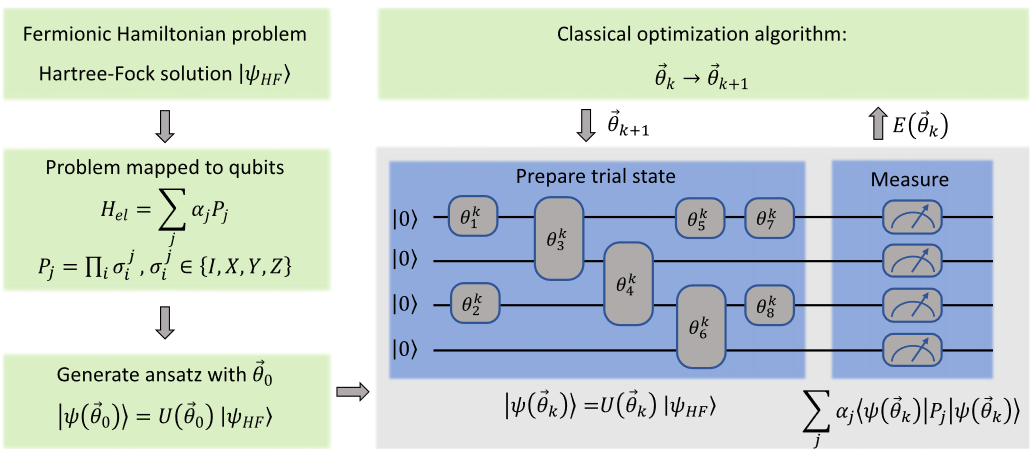
\includegraphics[width=0.8\textwidth]{figures/S3/flujovqe.png}
\caption{\label{fig:101} Flujo de trabajo del método \textit{variational quantum eigensolver}. Fuente: \cite{Fedorov2022}}
\end{figure}

\underline{\textit{Variational quantum deflation}}: 
La implementación del VQD sigue una estructura similar a la del VQE, con la diferencia que dentro del cálculo de la función de coste se considera un esquema de cálculo similar a la figura \ref{fig:102}. Para la función de coste ingresada se adapta para agregar el término de penalización, lo cual, agrega un coste adicional de listas para almacenar los parámetros de cada vector propio.

Para el cálculo del término de \textit{overlap} (penalización) se utiliza la expresión $U(\theta_k)U^{\dag}(\theta_i)$ con $i<k$, es decir, al \textit{ansatz} con los nuevos parámetros le añadimos el mismo \textit{ansatz} pero con la secuencia de términos invertidas y con los parámetros de uno de los estados anteriores. La idea es que, si volvemos al estado original, eso quiere decir que ambos estados son iguales y se tiene que penalizar.

La implementación solo puede ser utilizada en la combinación sistemas de espines con \textit{hardware efficient ansatz}.
\begin{figure}[H]
\centering
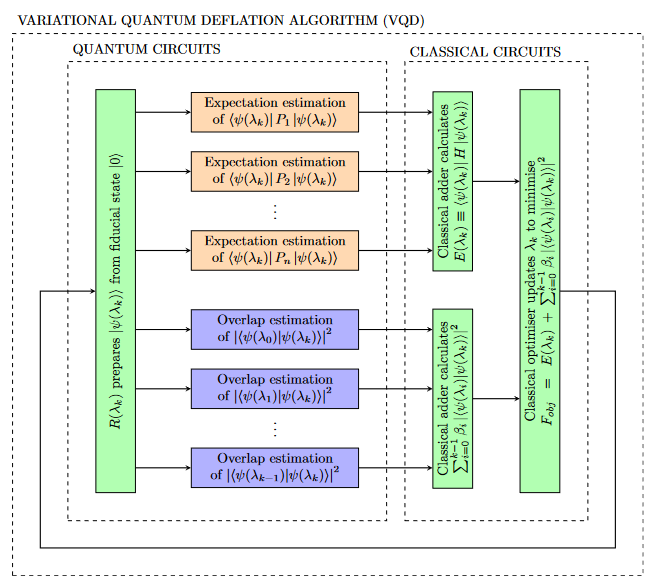
\includegraphics[width=0.75\textwidth]{figures/S3/flujovqd.png}
\caption{\label{fig:102} Flujo de trabajo del método \textit{variational quantum deflation}. Fuente: \cite{Higgott2019variationalquantum}}
\end{figure}




\subsubsection{Flujo de trabajo}
Finalmente, en esta última sección, se presentará un esquema general de los flujos de trabajo, junto con las subetapas. El flujo general se compone de 4 etapas, ver figura \ref{fig:110}, las cuales son independientes de los tipos de \textit{ansatz}, hamiltoniano, optimizador y método que se elijan. Cada una de estas etapas corresponde a la construcción de las tres clases mencionadas al inicio del capítulo, cada subetapa reflejas las operaciones que ocurren dentro de la clase y las que tienen que ser llamadas por el usuario.

\begin{figure}[H]
\centering
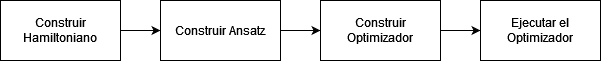
\includegraphics[width=0.8\textwidth]{figures/S3/flujogeneral.png}
\caption{\label{fig:110} Esquema general del flujo de trabajo. Fuente: Elaboración propia}
\end{figure}

La primera etapa está compuesta a su vez de 6 subetapas, ver figura \ref{fig:111}, la idea es un tipo de hamiltoniano y construirlo. Primero, se elige el tipo de hamiltoniano, ya que, de esa elección dependen los parámetros que se tienen que definir, una vez se tienen los parámetros, estos son utilizados para ejecutar funciones de las librerías que permiten construir los elementos básicos que son utilizados en la construcción de los hamiltonianos en el espacio de espines (en la representación propia de la librería), un detalle es que varias de las funciones utilizadas construyen términos de con constantes 0 (es decir, la constante que acompaña los términos es 0), por lo tanto, es menester aplicar un filtro que permite eliminar estos términos. Ahora que se tienen todos los términos, se utiliza la función para agrupar los términos conmutantes. Con lo anterior, tenemos un hamiltoniano expresado de una forma que nos permite realizar ejecuciones eficientes, los pasos siguientes consisten en reescribir estos grupos en la representación de lista de cadenas de Pauli y generar el representante de los grupos (este representante no es otra cosa que una cadena de caracteres, que nos indica que operador se encuentra en cada posición, este se utiliza para realizar los cambios de base correspondientes a cada \textit{qubit} a la hora de ejecutar los circuitos).

\begin{figure}[H]
\centering
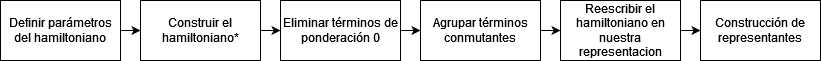
\includegraphics[width=0.99\textwidth]{figures/S3/flujo1.png}
\caption{\label{fig:111} Flujo de trabajo para construir el hamiltoniano del sistema. Fuente: Elaboración propia}
\end{figure}


La segunda etapa se compone de 4 subetapas, ver figura \ref{fig:112}, lo primero es definir los parámetros del \textit{ansatz}. Una vez hecho esto, se tiene que definir el \textit{backend} del \textit{ansatz} (el \textit{backend} contiene todas las configuraciones en las cuales se ejecutara el circuito), el siguiente es el simulador, en donde se ejecuta el circuito junto a las condiciones definidas \textit{backend} (modelos de ruido entre otros). Finalmente, el último elemento es el estado inicial del circuito, cabe mencionar, que este estado inicial no es el de los parámetros de las compuertas, es con el que se inicializa el circuito y al que después se le aplica el \textit{ansatz}.

\begin{figure}[H]
\centering
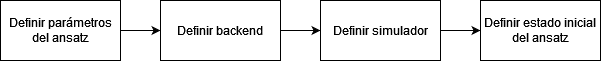
\includegraphics[width=0.9\textwidth]{figures/S3/flujo2.png}
\caption{\label{fig:112} Flujo de trabajo para construir el \textit{ansatz}. Fuente: Elaboración propia}
\end{figure}

La tercera etapa se compone de 3 subetapas, ver figura \ref{fig:113}, la idea de etapa es definir el optimizador que se va a utilizar para minimizar la función de coste. Entonces, lo primero es elegir el optimizador, uno de los optimizadores disponibles (ADAM y un método de gradiente genérico), en la práctica, los parámetros son los mismos para cada optimizador, por lo tanto, independiente de la selección, se tienen que definir los mismos parámetros. Una vez hecho esto, se construye la clase del optimizador.

\begin{figure}[H]
\centering
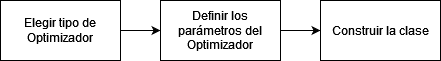
\includegraphics[width=0.7\textwidth]{figures/S3/flujo3.png}
\caption{\label{fig:113} Flujo de trabajo para construir el optimizador. Fuente: Elaboración propia}
\end{figure}

Finalmente, la cuarta etapa consiste en tomar la función de coste de la clase del hamiltoniano y ejecutar el optimizador (es decir, ejecutar el VQE o el VQD). Todo lo anterior es aplicable a cualquiera de las combinaciones que se definieron anteriormente, este flujo corresponde a un estándar para trabajar con los métodos variacionales cuánticos.

